% !TEX root = ../pdf/lsj.tex
% [There are multiple lsj.tex files, but the one in ../pdf is the usual one]



% to be added: something on how to use mean substitution in scales when scale items have missing values - see FLQ-NO.omv for example

\chapter{Pragmatic matters~\label{ch:datahandling}}

\begin{quote}
{\it The garden of life never seems to confine itself to the plots philosophers have
laid out for its convenience. Maybe a few more tractors would do the trick.} \\ \hspace*{2cm} -- Roger Zelazny\FOOTNOTE{The quote comes from {\it Home is the Hangman}, published in 1975.}
\end{quote}


\noindent
This is a somewhat strange chapter, even by my standards. My goal in this chapter is to talk a bit more honestly about the realities of working with data than you'll see anywhere else in the book. The problem with real world data sets is that they are {\it messy}. Very often the data file that you start out with doesn't have the variables stored in the right format for the analysis you want to do. Sometimes there might be a lot of missing values in your data set. Sometimes you only want to analyse a subset of the data. Et cetera. In other words, there's a lot of \keyterm{data manipulation} that you need to do, just to get the variables in your data set into the format that you need it. The purpose of this chapter is to provide a basic introduction to all these pragmatic topics. Although the chapter is motivated by the kinds of practical issues that arise when manipulating real data, I'll stick with the practice that I've adopted through most of the book and rely on very small, toy data sets that illustrate the underlying issue. Because this chapter is essentially a collection of techniques and doesn't tell a single coherent story, it may be useful to start with a list of topics:
\begin{itemize} \itemsep 0pt
\item Section~\ref{sec:freqtables}. Tabulating data.
\item Section~\ref{sec:transform}. Transforming or recoding a variable.
\item Section~\ref{sec:mathfunc}. Some useful mathematical functions.
\item Section~\ref{sec:subset}. Extracting a subset of a vector.
\item Section~\ref{sec:subsetdataframe}. Extracting a subset of a data frame.
\item Section~\ref{sec:sort}. Sorting, flipping or merging data sets.
\item Section~\ref{sec:reshape}. Reshaping a data frame.
\item Section~\ref{sec:textprocessing}. Manipulating text.
\item Section~\ref{sec:importing}. Opening data from different file types.
\item Section~\ref{sec:coercion}. Coercing data from one type to another.
\item Section~\ref{sec:datastructures}. Other important data types.
\item Section~\ref{sec:miscdatahandling}. Miscellaneous topics.
\end{itemize}
As you can see, the list of topics that the chapter covers is pretty broad, and there's a {\it lot} of content there. Even though this is one of the longest and hardest chapters in the book, I'm really only scratching the surface of several fairly different and important topics. My advice, as usual, is to read through the chapter once and try to follow as much of it as you can. Don't worry too much if you can't grasp it all at once, especially the later sections. The rest of the book is only lightly reliant on this chapter, so you can get away with just understanding the basics. However, what you'll probably find is that later on you'll need to flick back to this chapter in order to understand some of the concepts that I refer to here.




\section{Tabulating and cross-tabulating data\label{sec:freqtables}}

A very common task when analysing data is the construction of frequency tables, or cross-tabulation of one variable against another. These tasks can be achieved in jamovi, and I'll illustrate how in this section. 

\SUBSECTION{Creating tables for single variables}

Let's start with a simple example. As the father of a small child, I naturally spend a lot of time watching TV shows like {\it In the Night Garden}. In the \filename{nightgarden.csv} file, I've transcribed a short section of the dialogue. The file contains two variables of interest, \rtext{speaker} and \rtext{utterance}. Open up this data set in jamovi and take a look at the data in the `spreadsheet' view. You will see that the data looks something like this:

\noindent
`speaker' variable: \\
\rtext{upsy-daisy upsy-daisy upsy-daisy upsy-daisy tombliboo tombliboo makka-pakka makka-pakka makka-pakka makka-pakka} \\ \\
\noindent
`utterance' variable: \\
\rtext{pip pip onk onk ee oo pip pip onk onk} \\

and looking at this it becomes very clear what happened to my sanity! With these as my data, one task I might find myself needing to do is construct a frequency count of the number of words each character speaks during the show. The jamovi `Descriptives' screen has a check box called `Frequency tables' which does just this, see Figure \ref{fig:freqtable}. \\


\begin{figure}[h!!]
\begin{center}
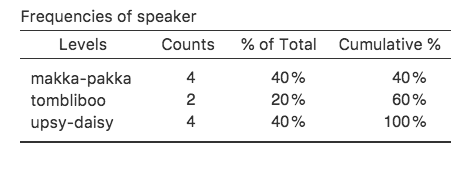
\epsfig{file = ../img/mechanics/freqtable.png, clip=true,width =12cm} 
\caption{Frequency table for the \rtext{speaker} variable}
\label{fig:freqtable}
\HR
\end{center}
\end{figure}

The output here tells us on the first line that what we're looking at is a tabulation of the \rtext{speaker} variable. In the `Levels' column it lists all the different speakers that exist in the data, and in the `Counts' column it tells you how many times that speaker appears in the data. In other words, it's a frequency table. 

In jamovi, the `Frequency tables' check box will only produce a table for single variables. For a table of two variables, for example combining \rtext{speaker} and \rtext{utterance}, so that we can see how many times each speaker said a particular utterance, we need a cross-tabulation or contingency table. In jamovi you can do this by selecting the `Frequencies' - `Contingency Tables' - `Independent Samples' analysis, and moving the \rtext{speaker} variable into the `Rows' box, and the \rtext{utterances} variable into the `Columns' box. You then should have a contingency table like the one shown in Figure \ref{fig:contingencytable}. \\


\begin{figure}[h!!]
\begin{center}
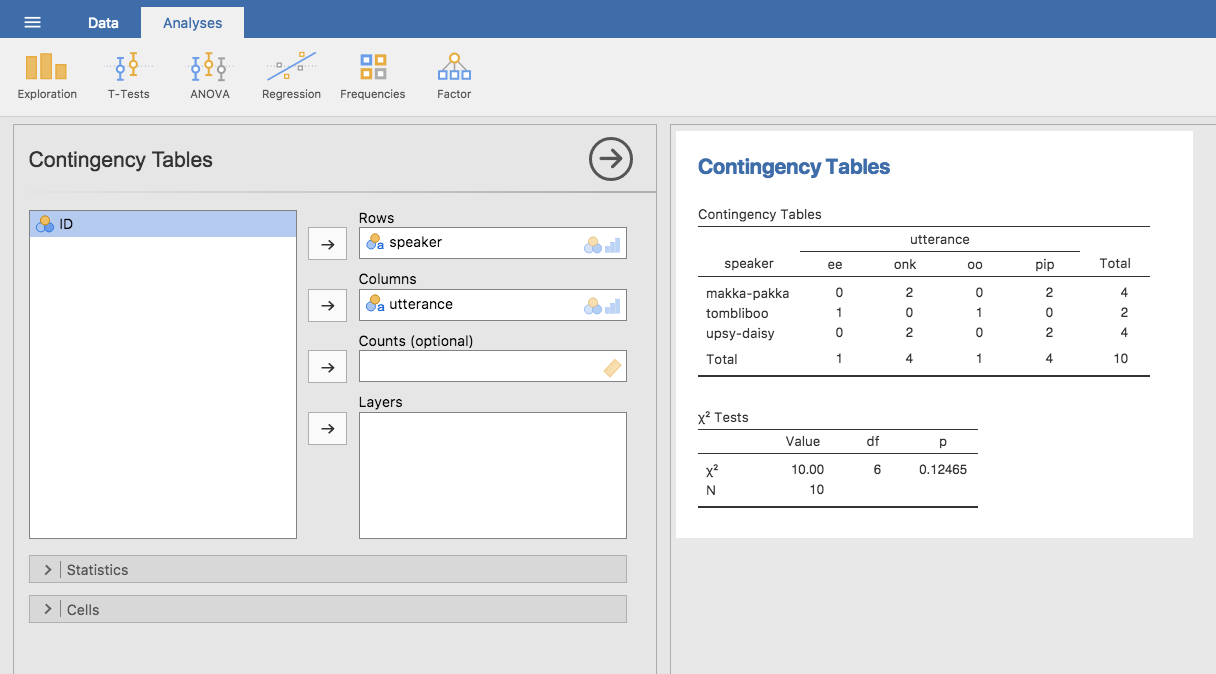
\epsfig{file = ../img/mechanics/contingencytable.png, clip=true,width =12cm} 
\caption{Contingency table for the \rtext{speaker} and \rtext{utterances} variables}
\label{fig:contingencytable}
\HR
\end{center}
\end{figure}

Don't worry about the ``$\chi^2$ Tests'' table that is produced, we are going to cover this later on in chapter \ref{ch:chisquare}. When interpreting the contingency table remember that these are counts: so the fact that the first row and second column of numbers corresponds to a value of 2 indicates that Makka-Pakka (row 1) says ``onk'' (column 2) twice in this data set. 


\SUBSECTION{Adding percentages to a contingency table}

The contingency table shown in Figure \ref{fig:contingencytable} shows a table of raw frequencies: that is, a count of the total number of cases for different combinations of levels of the specified variables. However, often you want your data to be organised in terms of percentages as well as counts. You can find the check boxes for different percentages under the `Cells' options in the `Contingency Tables' window. First, click on the `Row' check box and the Contingency Table in the output window will change to the one in Figure \ref{fig:contingencyrow}. 

\begin{figure}[h!!]
\begin{center}
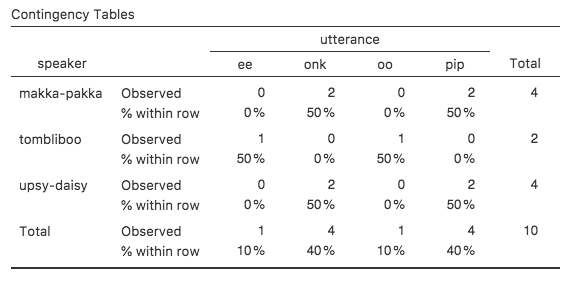
\epsfig{file = ../img/mechanics/contingencyrow.png, clip=true,width =12cm} 
\caption{Contingency table for the \rtext{speaker} and \rtext{utterances} variables, with row percentages}
\label{fig:contingencyrow}
\HR
\end{center}
\end{figure}

What we're looking at here is the percentage of utterances made by each character. In other words, 50\% of Makka-Pakka's utterances are ``pip'', and the other 50\% are ``onk''. Let's contrast this with the table we get when we calculate column percentages (uncheck `Row' and check `Column' in the Cells options window), see Figure \ref{fig:contingencycol}. In this version, what we're seeing is the percentage of characters associated with each utterance. For instance, whenever the utterance ``ee'' is made (in this data set), 100\% of the time it's a Tombliboo saying it. 

\begin{figure}[h!!]
\begin{center}
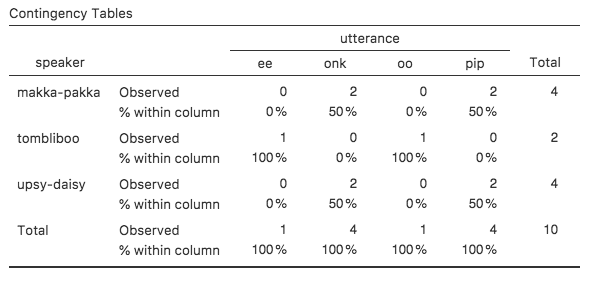
\epsfig{file = ../img/mechanics/contingencycol.png, clip=true,width =12cm} 
\caption{Contingency table for the \rtext{speaker} and \rtext{utterances} variables, with column percentages}
\label{fig:contingencycol}
\HR
\end{center}
\end{figure}



%%%%%%%%%%%%%%%%% next section copied from original ch. 3


\section{Logical expressions in jamovi\label{sec:logicals}}

A key concept that a lot of data transformations in jamovi rely on is the idea of a \keyterm{logical value}. A logical value is an assertion about whether something is true or false. This is implemented in jamovi in a pretty straightforward way. There are two logical values, namely \rtext{TRUE} and \rtext{FALSE}. Despite the simplicity, logical values are very useful things. Let's see how they work.

\SUBSECTION{Assessing mathematical truths}

In George Orwell's classic book {\it 1984}, one of the slogans used by the totalitarian Party was ``two plus two equals five'', the idea being that the political domination of human freedom becomes complete when it is possible to subvert even the most basic of truths. It's a terrifying thought, especially when the protagonist Winston Smith finally breaks down under torture and agrees to the proposition. ``Man is infinitely malleable'', the book says. I'm pretty sure that this isn't true of humans\FOOTNOTE{I offer up my teenage attempts to be ``cool'' as evidence that some things just can't be done.} but it's definitely not true of jamovi. jamovi is not infinitely malleable - it has rather firm opinions on the topic of what is and isn't true, at least as regards basic mathematics. If I ask it to calculate \rtext{2 + 2}\FOOTNOTE{You can do this in the Compute new variable screen, though just calculating 2 + 2 for every cell of a new variable is not very useful!}, it always gives the same answer, and it's not bloody 5!

Of course, so far jamovi is just doing the calculations. I haven't asked it to explicitly assert that $2+2 = 4$ is a true statement. If I want jamovi to make an explicit judgement, I can use a command like this: \rtext{2 + 2 == 4}

What I've done here is use the \keyterm{equality operator}, \rtext{==}, to force jamovi to make a ``true or false'' judgement.\FOOTNOTE{Note that this is a very different operator to the equals operator \rtextsmall{=}. A common typo that people make when trying to write logical commands in jamovi (or other languages, since the ``\rtextsmall{=} versus \rtextsmall{==}'' distinction is important in many computer and statistical programmes) is to accidentally type \rtextsmall{=} when you really mean \rtextsmall{==}. Be especially cautious with this -- I've been programming in various languages since I was a teenager, and I {\it still} screw this up a lot. Hm. I think I see why I wasn't cool as a teenager. And why I'm still not cool.} Okay, let's see what jamovi thinks of the Party slogan, so type this into the compute new variable `formula' box: 

\begin{rblock1}
2 + 2 == 5
\end{rblock1}

...and what do you get - it should be a whole set of `false' values in the spreadsheet column for your newly computed variable. Booyah! Freedom and ponies for all! Or something like that. Anyway, it's worth having a look at what happens if I try to {\it force} jamovi to believe that two plus two is five by making an statement like  \rtext{2 + 2 = 5}. I know that if I do this in another programme, say \R\, then it throws up an error message. But wait, if you do this in jamovi you still get a whole set of `false' values. So what is going on...well it seems that jamovi is being pretty smart, and realises that you are testing whether it is TRUE or FALSE that \rtext{2 + 2 = 5} regardless of whether you use the correct \keyterm{equality operator}, \rtext{==}, or the equals sign ``=''. 

\SUBSECTION{Logical operations}
%\index{R}{{<}}
%\index{R}{{<=}}
%\index{R}{{>=}}
%\index{R}{{!=}}

So now we've seen logical operations at work, but so far we've only seen the simplest possible example. You probably won't be surprised to discover that we can combine logical operations with other operations and functions in a more complicated way, like this:

\begin{rblock1}
3*3 + 4*4 == 5*5
\end{rblock1} 

or this

\begin{rblock1}
SQRT( 25 ) == 5
\end{rblock1}

Not only that, but as Table~\ref{tab:logicals} illustrates, there are several other logical operators that you can use, corresponding to some basic mathematical concepts. Hopefully these are all pretty self-explanatory: for example, the \keyterm{less than} operator \rtext{<} checks to see if the number on the left is less than the number on the right. If it's less, then jamovi returns an answer of \rtextoutput{TRUE}, but if the two numbers are equal, or if the one on the right is larger, then jamovi returns an answer of \rtextoutput{FALSE}.

In contrast, the \keyterm{less than or equal to} operator \rtextverb#<=# will do exactly what it says. It returns a value of \rtextoutput{TRUE} if the number of the left hand side is less than or equal to the number on the right hand side. At this point I hope it's pretty obvious what the \keyterm{greater than} operator \rtext{>} and the \keyterm{greater than or equal to} operator \rtextverb#>=# do! 

Next on the list of logical operators is the \keyterm{not equal to} operator \rtextverb#!=# which -- as with all the others -- does what it says it does. It returns a value of \rtext{TRUE} when things on either side are not identical to each other. Therefore, since $2+2$ isn't equal to $5$, we would get `true' as the value for our newly computed variable. Try it and see:

\begin{rblock1}
2 + 2 != 5
\end{rblock1}


\begin{table}
\caption{Some logical operators. Technically I should be calling these ``binary relational operators'', but quite frankly I don't want to. It's my book so no-one can make me.} \tabcapsep
\label{tab:logicals}
\begin{center}
\begin{tabular}{lc|cc}
operation  				& operator 	& example input 	& answer \\ \hline
less than  				&\rtextverb#<# 	& \rtextverb#2 < 3# 	& \rtextoutput{TRUE} \\
less than or equal to	&\rtextverb#<=#	& \rtextverb#2 <= 2#	& \rtextoutput{TRUE} \\
greater than				&\rtextverb#>#	& \rtextverb#2 > 3# 	& \rtextoutput{FALSE}\\
greater than or equal to	&\rtextverb#>=#	& \rtextverb#2 >= 2# & \rtextoutput{TRUE} \\ 
equal to			&\rtextverb#==#	& \rtextverb#2 == 3# & \rtextoutput{FALSE}\\
not equal to				&\rtextverb#!=#	& \rtextverb#2 != 3# & \rtextoutput{TRUE} \\
\end{tabular}
\tabcapsep \HR
\end{center}
\end{table}

\begin{table}
\caption{Some more logical operators.} \tabcapsep
\label{tab:logicals2}
\begin{center}
\begin{tabular}{lc|cc} 
operation  				& operator 	& example input 	& answer \\ \hline
not 						&\rtextverb#NOT#	& \rtextverb#NOT(1==1)# & \rtextoutput{FALSE} \\ 
or 						&\rtextverb#or#	& \rtextverb#(1==1) or (2==3)# & \rtextoutput{TRUE} \\
and 						&\rtextverb#and# &\rtextverb#(1==1) and (2==3)# & \rtextoutput{FALSE} \\ 
\end{tabular}
\tabcapsep \HR
\end{center}
\end{table}

We're not quite done yet. There are three more logical operations that are worth knowing about, listed in Table~\ref{tab:logicals2}. These are the \keyterm{not} operator \rtextverb#!#, the \keyterm{and} operator \rtextverb#and#, and the \keyterm{or} operator \rtextverb#or#. Like the other logical operators, their behaviour is more or less exactly what you'd expect given their names. For instance, if I ask you to assess the claim that ``either $2+2 = 4$ {\it or} $2+2 = 5$'' you'd say that it's true. Since it's an ``either-or'' statement, all we need is for one of the two parts to be true. That's what the \rtext{or} operator does:\FOOTNOTE{Now, here's a quirk in jamovi. When you have simple logical expressions like the ones we have already met, e.g. \rtext{2 + 2 == 5} then jamovi neatly states `false' (or `true') in the corresponding spreadsheet column. Underneath the hood, jamovi stores `false' as \rtext{0} and `true' as \rtext{1}. When we have more complex logical expressions, such as \rtext{(2+2 == 4) or (2+2 == 5)}, then jamovi just displays either \rtext{0} or \rtext{1}, depending whether the logical expression is evaluated as false, or true. }

\begin{rblock1}
(2+2 == 4) or (2+2 == 5) 
\end{rblock1}

On the other hand, if I ask you to assess the claim that ``both $2+2 = 4$ {\it and} $2+2 = 5$'' you'd say that it's false. Since this is an {\it and} statement we need both parts to be true. And that's what the \rtextverb#and# operator does:

\begin{rblock1}
(2+2 == 4) and (2+2 == 5)
\end{rblock1}

Finally, there's the {\it not} operator, which is simple but annoying to describe in English. If I ask you to assess my claim that ``it is not true that $2+2 = 5$'' then you would say that my claim is true; because my claim is that ``$2+2 = 5$ is false''. And I'm right. If we write this in jamovi we get this: 

\begin{rblock1}
NOT(2+2 == 5)
\end{rblock1}

In other words, since \rtext{2+2 == 5} is a \rtext{FALSE} statement, it must be the case that \rtext{NOT(2+2 == 5)} is a \rtext{TRUE} one. Essentially, what we've really done is claim that ``not false'' is the same thing as ``true''. Obviously, this isn't really quite right in real life. But jamovi lives in a much more black or white world: for jamovi everything is either true or false. No shades of gray are allowed. 

Of course, in our $2+2 = 5$ example, we didn't really need to use ``not'' \rtext{NOT} and ``equals to'' \rtext{==} as two separate operators. We could have just used the ``not equals to'' operator \rtext{!=} like this:

\begin{rblock1}
{2+2 != 5}
\end{rblock1}

\SUBSECTION{Applying logical operation to text~\label{sec:logictext}}

I also want to briefly point out that you can apply these logical operators to text as well as to logical data. It's just that we need to be a bit more careful in understanding how jamovi interprets the different operations. In this section I'll talk about how the equal to operator \rtext{==} applies to text, since this is the most important one. Obviously, the not equal to operator \rtext{!=} gives the exact opposite answers to \rtext{==} so I'm implicitly talking about that one too, but I won't give specific commands showing the use of \rtext{!=}. As for the other operators, I'll defer a more detailed discussion of this topic to Section~\ref{sec:logictext2}. 

Okay, let's see how it works. In one sense, it's very simple. For instance, I can ask jamovi if the word \rtext{"cat"} is the same as the word 
\rtext{"dog"}, like this:

\begin{rblock1}
"cat" == "dog"
\end{rblock1}

That's pretty obvious, and it's good to know that even jamovi can figure that out. Similarly, jamovi does recognise that a \rtext{"cat"} is a \rtext{"cat"}:

\begin{rblock1}
"cat" == "cat"
\end{rblock1}

Again, that's exactly what we'd expect. However, what you need to keep in mind is that jamovi is not at all tolerant when it comes to grammar and spacing. If two strings differ in any way whatsoever, jamovi will say that they're not equal to each other, as with the following: 

\begin{rblock1}
" cat" == "cat"
"cat" == "CAT""cat" == "c a t"
\end{rblock1}

You can also use other logical operators too. For instance jamovi also allows you to use the \rtext{<} and \rtext{>} operators to determine which of two text `strings' comes first, alphabetically speaking. Sort of. Actually, it's a bit more complicated than that, but let's start with a simple example:

\begin{rblock1}
"cat" < "dog"
\end{rblock1}

In jamovi, this example evaluates to `true'. This is because \rtext{"cat"} does does come before \rtext{"dog"} alphabetically, so jamovi judges the statement to be true. However, if we ask jamovi to tell us if \rtext{"cat"} comes before \rtext{"anteater"} then it will evaluate the expression as false. So far, so good. But text data is a bit more complicated than the dictionary suggests. What about \rtext{"cat"} and \rtext{"CAT"}? Which of these comes first? Try it and find out:

\begin{rblock1}
"CAT" < "cat"
\end{rblock1}

This in fact evaluates to `true'. In other words, jamovi assumes that uppercase letters come before lowercase ones. Fair enough. No-one is likely to be surprised by that. What you might find surprising is that jamovi assumes that {\it all} uppercase letters come before {\it all} lowercase ones. That is, while \rtext{"anteater" < "zebra"} is a true statement, and the uppercase equivalent \rtext{"ANTEATER" < "ZEBRA"} is also true, it is {\it not} true to say that \rtext{"anteater" < "ZEBRA"}, as the following extract illustrates. Try this: 

\begin{rblock1}
"anteater" < "ZEBRA"
\end{rblock1}

This evaluates to `false', and this may seem slightly counterintuitive. With that in mind, it may help to have a quick look Table~\ref{tab:asciiorder}, which lists various text characters in the order that jamovi uses. 

\begin{table}
\begin{center}
\caption{The ordering of various text characters used by the \rtext{<} and \rtext{>} operators. Not shown is the ``space'' character, which actually comes first on the list.}\tabcapsep
\label{tab:asciiorder}
\begin{verbatim}
            ! " # $ % & ' ( ) * + , - . /  0 1 2 3 4 5 6 7 8 9 : ; < = > ? @ 
            A B C D E F G H I J K L M N O P Q R S T U V W X Y Z [ \ ]  ^ _ ` 
            a b c d e f g h i j k l m n o p q r s t u v w x y z } | {
\end{verbatim}
\HR
\end{center}
\end{table}



\section{Transforming and recoding a variable~\label{sec:transform}}

It's not uncommon in real world data analysis to find that one of your variables isn't quite equivalent to the variable that you really want. For instance, it's often convenient to take a continuous-valued variable (e.g., age) and break it up into a smallish number of categories (e.g., younger, middle, older). At other times, you may need to convert a numeric variable into a different numeric variable (e.g., you may want to analyse at the absolute value of the original variable). In this section I'll describe a few key ways you can do these things in jamovi. 


\SUBSECTION{Creating a transformed variable}

The first trick to discuss is the idea of \keyterm{transforming} a variable. Taken literally, {\it anything} you do to a variable is a transformation, but in practice what it usually means is that you apply a relatively simple mathematical function to the original variable, in order to create a new variable that either (a) provides a better way of describing the thing you're actually interested in or (b) is more closely in agreement with the assumptions of the statistical tests you want to do.  Since -- at this stage -- I haven't talked about statistical tests or their assumptions, I'll show you an example based on the first case. 

Suppose I've run a short study in which I ask 10 people a single question: 
\begin{quote}
On a scale of 1 (strongly disagree) to 7 (strongly agree), to what extent do you agree with the proposition that ``Dinosaurs are awesome''?
\end{quote}
Now let's load and look at the data. The data file \filename{likert.omv} contains a single variable that contains raw Likert-scale responses for these 10 people. However, if you think about it, this isn't the best way to represent these responses. Because of the fairly symmetric way that we set up the response scale, there's a sense in which the midpoint of the scale should have been coded as 0 (no opinion), and the two endpoints should be $+3$ (strong agree) and $-3$ (strong disagree). By recoding the data in this way, it's a bit more reflective of how we really think about the responses. The recoding here is trivially easy: we just subtract 4 from the raw scores, and in jamovi you can do this by computing a new variable: click on the `Data' - `Compute' button and you will see that a new variable has been added to the spreadsheet. Let's call this new variable \rtext{likert.centered} (go ahead and type that in) and then add the following in the formula box, like in Figure \ref{fig:likertraw}: \\ 

\rtext{likert.raw - 4} \\

\begin{figure}[h!!]
\begin{center}
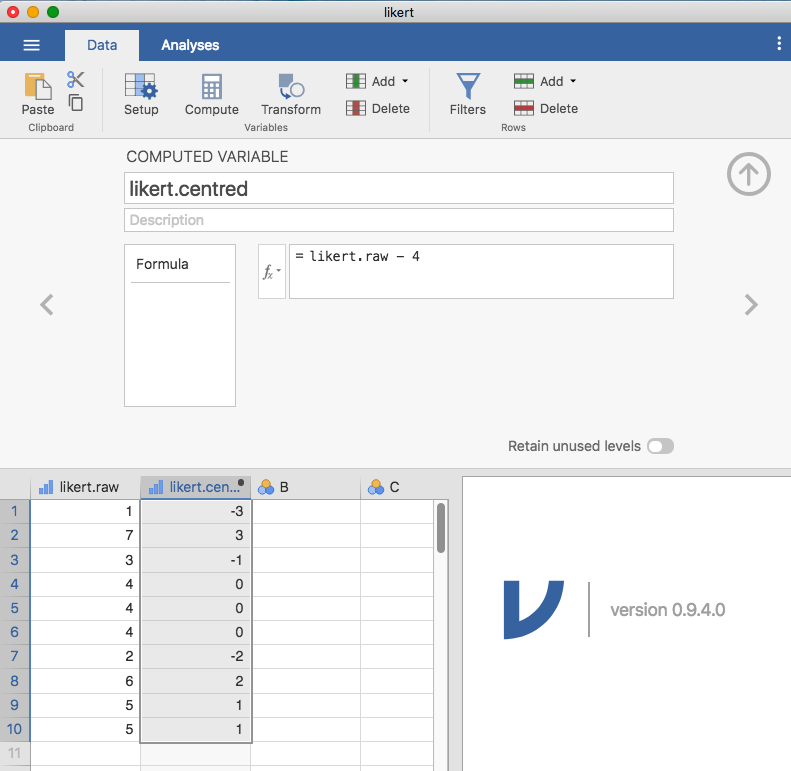
\epsfig{file = ../img/mechanics/likertraw.png, clip=true,width =12cm} 
\caption{Creating a new computed variable in jamovi}
\label{fig:likertraw}
\HR
\end{center}
\end{figure}

One reason why it might be useful to have the data in this format is that there are a lot of situations where you might prefer to analyse the {\it strength} of the opinion separately from the {\it direction} of the opinion. We can do two different transformations on this \rtext{likert.centered} variable in order to distinguish between these two different concepts. Firstly, to compute an \rtext{opinion.strength} variable, we want to take the absolute value of the centered data (using the `ABS' function). In jamovi, create another new variable using the `Compute' button. Name the variable \rtext{opinion.strength} and this time click on the {\it f\textsubscript{x}} button next to the function box. This shows the different `Functions' and `Variables' that you can add to the function box, so double click on `ABS' and then double click on ``likert.centered' and you will see that the function box is populated with ABS(likert.centered) and a new variable has been created in the spreadsheet view, as in Figure \ref{fig:opinionstrength}

\begin{figure}[h!!]
\begin{center}
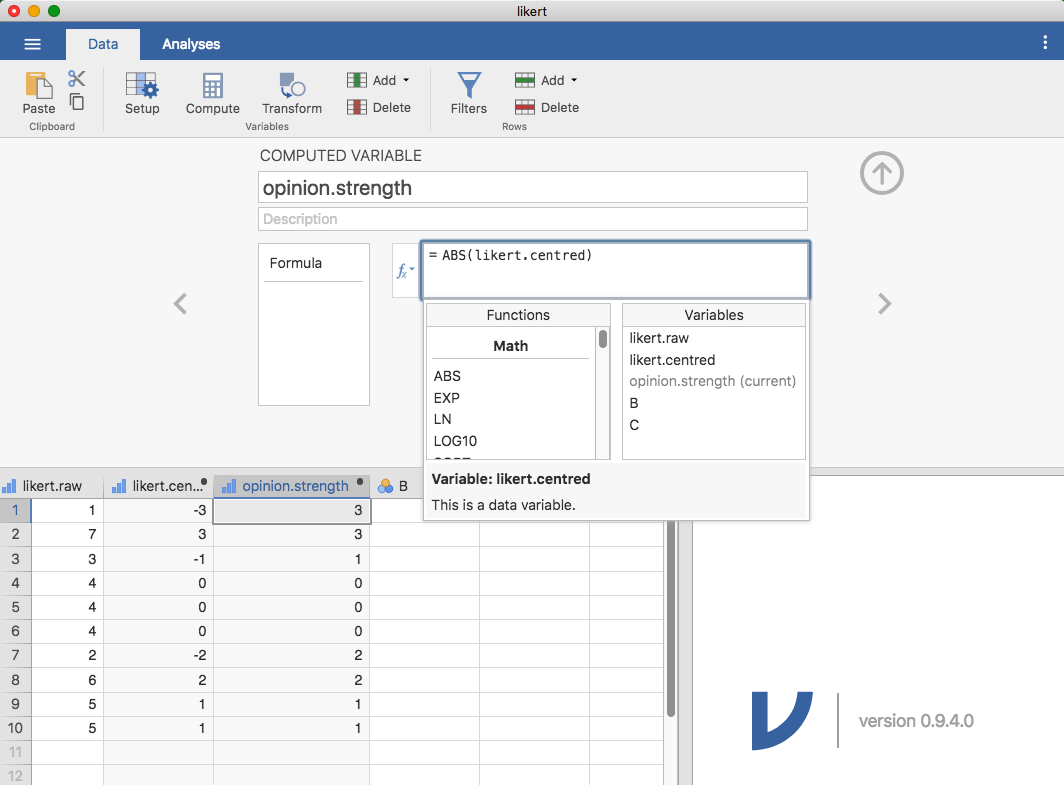
\epsfig{file = ../img/mechanics/opinionstrength.png, clip=true,width =12cm} 
\caption{Using the {\it f\textsubscript{x}} button to select functions and variables}
\label{fig:opinionstrength}
\HR
\end{center}
\end{figure}


Secondly, to compute a variable that contains only the direction of the opinion and ignores the strength, we want to calculate the `sign' of the variable. In jamovi we can use the \rtext{IF} function to do this, so create another new variable using the `Compute' button, name this one \rtext{opinion.sign}, and then type the following into the function box: \\


\rtext{IF(likert.centered == 0, 0, likert.centered / opinion.strength)} \\


When done, you'll see that all negative numbers from the \rtext{likert.centered} variable are converted to $-1$, all positive numbers are converted to $1$ and zero stays as $0$, like so: 

\begin{rblock1}
-1  1 -1  0  0  0 -1  1  1  1
\end{rblock1}

Let's break down what this `IF' command is doing. In jamovi, there are three parts to an `IF' statement, written as 'IF(expression, value, else)'. The first part, `expression' can be a logical or mathematical statement. In our example, we have specified `likert.centered == 0', meaning take all those values where likert.centered is zero. The next part, `value', gives a new value where the expression in part one is satisfied. In our example, we have said that for all those values where likert.centered is zero, keep them zero. In the next part, `else', we can enter another logical or mathematical statement to work on every other value apart from the value(s) we specified in part one, i.e. zero. In our example we have divided likert.centered by opinion.strength to give `-1' or `+1' depending of the sign of the original value in likert.centered\FOOTNOTE{The reason we have to use the `IF' command and keep zero as zero is that you cannot  just use likert.centered / opinion.strength to calculate the sign of likert.centered - because mathematically dividing zero by zero does not work - try it and see}.

And we're done. We now have three shiny new variables, all of which are useful transformations of the original \rtext{likert.raw} data. 



\SUBSECTION{Collapsing a variable into a smaller number of discrete levels or categories}

One pragmatic task that arises more often than you'd think is the problem of collapsing a variable into a smaller number of discrete levels or categories. For instance, suppose I'm interested in looking at the age distribution of people at a social gathering:\\
\begin{rblock1}
60,58,24,26,34,42,31,30,33,2,9
\end{rblock1}
In some situations it can be quite helpful to group these into a smallish number of categories. For example, we could group the data into three broad categories: young (0-20), adult (21-40) and older (41-60). This is a quite coarse-grained classification, and the labels that I've attached only make sense in the context of this data set (e.g., viewed more generally, a 42 year old wouldn't consider themselves as ``older''). We can slice this variable up quite easily using the jamovi `IF' function that we have already used. This time we have to specify nested `IF' statements, meaning simply that IF the first logical expression is TRUE, insert a first value, but IF a second logical expression is TRUE, insert a second value, but IF a third logical expression is TRUE, then insert a third value. This can be written as: \\ 

\noindent
\rtext{
IF(Age >= 0 and Age <= 20, 1, \\
IF(Age >= 21 and Age <= 40, 2, \\
IF(Age >= 41 and Age <= 60, 3 )))
} \\

Note that there are three left parentheses used during the nesting, so the whole statement has to end with three right parentheses, otherwise you will get an error message. The jamovi screen shot for this data manipulation, along with an accompanying frequency table, is shown in Figure \ref{fig:agecats} 



\begin{figure}[h!!]
\begin{center}
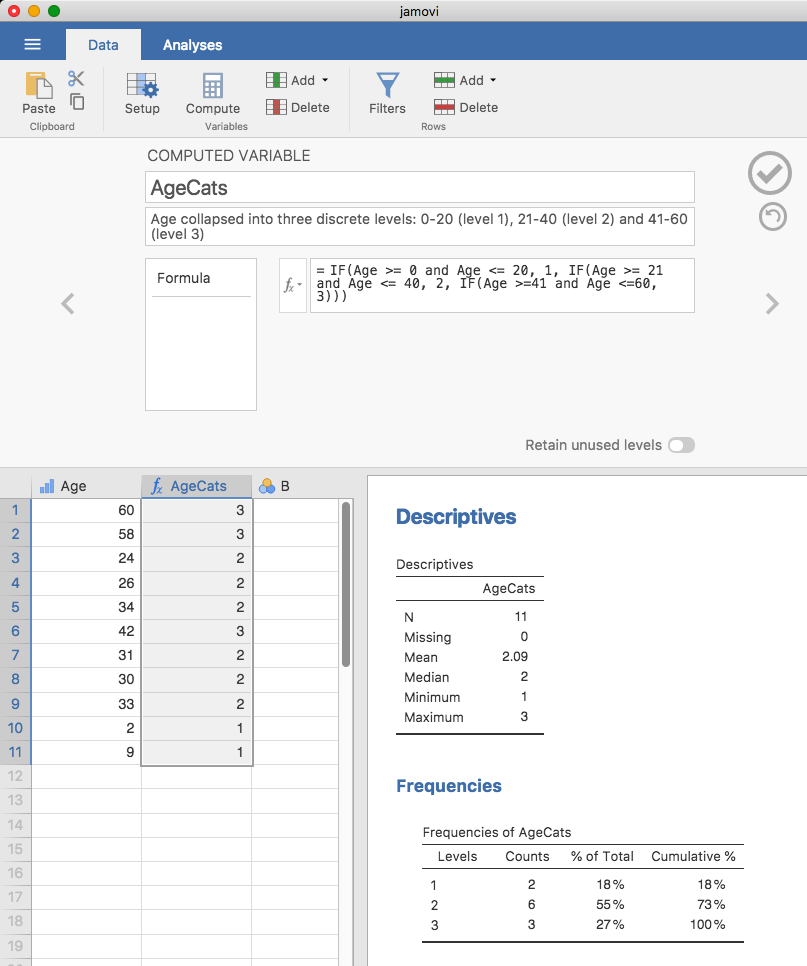
\epsfig{file = ../img/mechanics/agecats.png, clip=true,width =12cm} 
\caption{Collapsing a variable into a smaller number of discrete levels using the jamovi `IF' function}
\label{fig:agecats}
\HR
\end{center}
\end{figure}


It's important to take the time to figure out whether or not the resulting categories make any sense at all in terms of your research project. If they don't make any sense to you as meaningful categories, then any data analysis that uses those categories is likely to be just as meaningless. More generally, in practice I've noticed that people have a very strong desire to carve their (continuous and messy) data into a few (discrete and simple) categories; and then run analysis using the categorised data instead of the original one.\FOOTNOTE{If you've read further into the book, and are re-reading this section, then a good example of this would be someone choosing to do an ANOVA using \rtextsmall{AgeCats} as the grouping variable, instead of running a regression using \rtextsmall{Age} as a predictor. There are sometimes good reasons for do this: for instance, if the relationship between \rtextsmall{Age} and your outcome variable is highly non-linear, and you aren't comfortable with trying to run non-linear regression! However, unless you really do have a good rationale for doing this, it's best not to. It tends to introduce all sorts of other problems (e.g., the data will probably violate the normality assumption), and you can lose a lot of power.} I wouldn't go so far as to say that this is an inherently bad idea, but it does have some fairly serious drawbacks at times, so I would advise some caution if you are thinking about doing it. 


\section{A few more mathematical functions and operations~\label{sec:mathfunc}}

In Section~\ref{sec:transform} I discussed the ideas behind variable transformations, and showed that a lot of the transformations that you might want to apply to your data are based on fairly simple mathematical functions and operations. In this section I want to return to that discussion, and mention several other mathematical functions and arithmetic operations that are actually quite useful for a lot of real world data analysis. Table~\ref{tab:mathfunc} gives a brief overview of the various mathematical functions I want to talk about here. Obviously this doesn't even come close to cataloguing the range of possibilities available, but it does cover a range of functions that are used regularly in data analysis and that are available in jamovi.



\begin{table}
\begin{center}
\caption{Some of the mathematical functions available in jamovi} \tabcapsep
\label{tab:mathfunc}
\begin{tabular}{l|llr}
 		& function 	& example input 	& (answer)\\ \hline
square root 	&\rtext{SQRT(x)}	& \rtext{SQRT(25)}	& \rtextoutput{5} \\
absolute value & \rtext{ABS(x)} & \rtext{ABS(-23)} & \rtextoutput{23} \\
logarithm (base 10)	&\rtext{LOG10(x)}	& \rtext{LOG10(1000)}	& \rtextoutput{3} \\
logarithm (base $e$) &\rtext{LN(x)}	& \rtext{LN(1000)} & \rtextoutput{6.908} \\
exponentiation	& \rtext{EXP(x)}	& \rtext{EXP(6.908)} 	& \rtextoutput{1000.245}\\ 
box-cox & \rtext{BOXCOX(x, lamda)}	& \rtext{BOXCOX(6.908, 3)} 	& \rtextoutput{109.551}\\ 
%rounding to nearest & \rtext{round()} & \rtext{round(1.32)} & \rtextoutput{1} \\
%rounding down & \rtext{floor()} & \rtext{floor(1.32)} & \rtextoutput{1} \\
%rounding up & \rtext{ceiling()} & \rtext{ceiling(1.32)} & \rtextoutput{2} \\ 
\end{tabular}\tabcapsep \HR
\end{center}
\end{table} 


\SUBSECTION{Logarithms and exponentials}

%\index{R}{{log}}
%\index{R}{{exp}}

As I've mentioned earlier, jamovi has an useful range of mathematical functions built into it, and there really wouldn't be much point in trying to describe or even list all of them. For the most part, I've focused only on those functions that are strictly necessary for this book. However I do want to make an exception for logarithms and exponentials. Although they aren't needed anywhere else in this book, they are {\it everywhere} in statistics more broadly, and not only that, there are a {\it lot} of situations in which it is convenient to analyse the logarithm of a variable (i.e., to take a ``log-transform'' of the variable). I suspect that many (maybe most) readers of this book will have encountered logarithms and exponentials before, but from past experience I know that there's a substantial proportion of students who take a social science statistics class who haven't touched logarithms since high school, and would appreciate a bit of a refresher. 

In order to understand logarithms and exponentials, the easiest thing to do is to actually calculate them and see how they relate to other simple calculations. There are three jamovi functions in particular that I want to talk about, namely \rtext{LN()}, \rtext{LOG10()} and \rtext{EXP()}. To start with, let's consider \rtext{LOG10()}, which is known as the ``logarithm in base 10''. The trick to understanding a \keyterm{logarithm} is to understand that it's basically the ``opposite'' of taking a power. Specifically, the logarithm in base 10 is closely related to the powers of 10. So let's start by noting that 10-cubed is 1000. Mathematically, we would write this:
$$ 
10^3 = 1000
$$
The trick to understanding a logarithm is to recognise that the statement that ``10 to the power of 3 is equal to 1000'' is equivalent to the statement that ``the logarithm (in base 10) of 1000 is equal to 3''. Mathematically, we write this as follows,
$$
\log_{10}( 1000 ) = 3
$$

Okay, since the \rtext{LOG10()} function is related to the powers of 10, you might expect that there are other logarithms (in bases other than 10) that are related to other powers too. And of course that's true: there's not really anything mathematically special about the number 10. You and I happen to find it useful because decimal numbers are built around the number 10, but the big bad world of mathematics scoffs at our decimal numbers. Sadly, the universe doesn't actually care how we write down numbers. Anyway, the consequence of this cosmic indifference is that there's nothing particularly special about calculating logarithms in base 10. You could, for instance, calculate your logarithms in base 2. Alternatively, a third type of logarithm -- and one we see a lot more of in statistics than either base 10 or base 2 -- is called the \keyterm{natural logarithm}, and corresponds to the logarithm in base $e$. Since you might one day run into it, I'd better explain what $e$ is. The number $e$, known as \keyterm{Euler's number}, is one of those annoying ``irrational'' numbers whose decimal expansion is infinitely long, and is considered one of the most important numbers in mathematics. The first few digits of $e$ are:
$$
e = 2.718282 
$$ 
There are quite a few situation in statistics that require us to calculate powers of $e$, though none of them appear in this book. Raising $e$ to the power $x$ is called the \keyterm{exponential} of $x$, and so it's very common to see $e^x$ written as $\exp(x)$. And so it's no surprise that jamovi has a function that calculate exponentials, called \rtext{EXP()}. Because the number $e$ crops up so often in statistics, the natural logarithm (i.e., logarithm in base $e$) also tends to turn up. Mathematicians often write it as $\log_e(x)$ or $\ln(x)$, or sometimes even just $\log(x)$. In fact, jamovi works the same way: the \rtext{LN()} function corresponds to the natural logarithm.

And with that, I think we've had quite enough exponentials and logarithms for this book!

%%%%%%%%%%%%%%%%%%%%%%%%%%%%%%%%%%%%%%%%
%Rework this section to add in details about sqrt and boxcox and frame as useful for transforming skewed variables
%%%%%%%%%%%%%%%%%%%%%%%%%%%%%%%%%%%%%%%%






\section{Extracting a subset of the data~\label{sec:subset}}

One very important kind of data handling is being able to extract a particular subset of the data. For instance, you might be interested only in analysing the data from one experimental condition, or you may want to look closely at the data from people over 50 years in age. To do this, the first step is getting jamovi to filter the subset of the data corresponding to the observations that you're interested in. 

This section returns to the \filename{nightgarden.csv} data set. If you're reading this whole chapter in one sitting, then you should already have this data set loaded into a jamovi window. For this section, let's focus on the two variables \rtext{speaker} and \rtext{utterance} (see Section~\ref{sec:freqtables} if you've forgotten what those variables look like). Suppose that what I want to do is pull out only those utterances that were made by Makka-Pakka. To that end, we need to specify a filter in jamovi: first open up a filter window by clicking on `Filters' on the main jamovi `Data' toolbar. Then in the `Filter 1' text box, next to the `=' sign, type the following:

\begin{rblock1}
speaker == 'makka-pakka'
\end{rblock1}

When you have done this, you will see that a new column has been added to the spreadsheet window (see Figure \ref{fig:subset1}), labelled `Filter 1', with the cases where \rtext{speaker} \underline{is not} `makka-pakka' greyed-out (ie filtered out) and, conversely, the cases where \rtext{speaker} \underline{is} `makka-pakka'have a green check mark, indicating they are filtered in. You can test this by running `Exploration' - `Descriptives' - `Frequency tables' for the \rtext{speaker} variable and seeing what that shows - go on, try it!

\begin{figure}[h!!]
\begin{center}
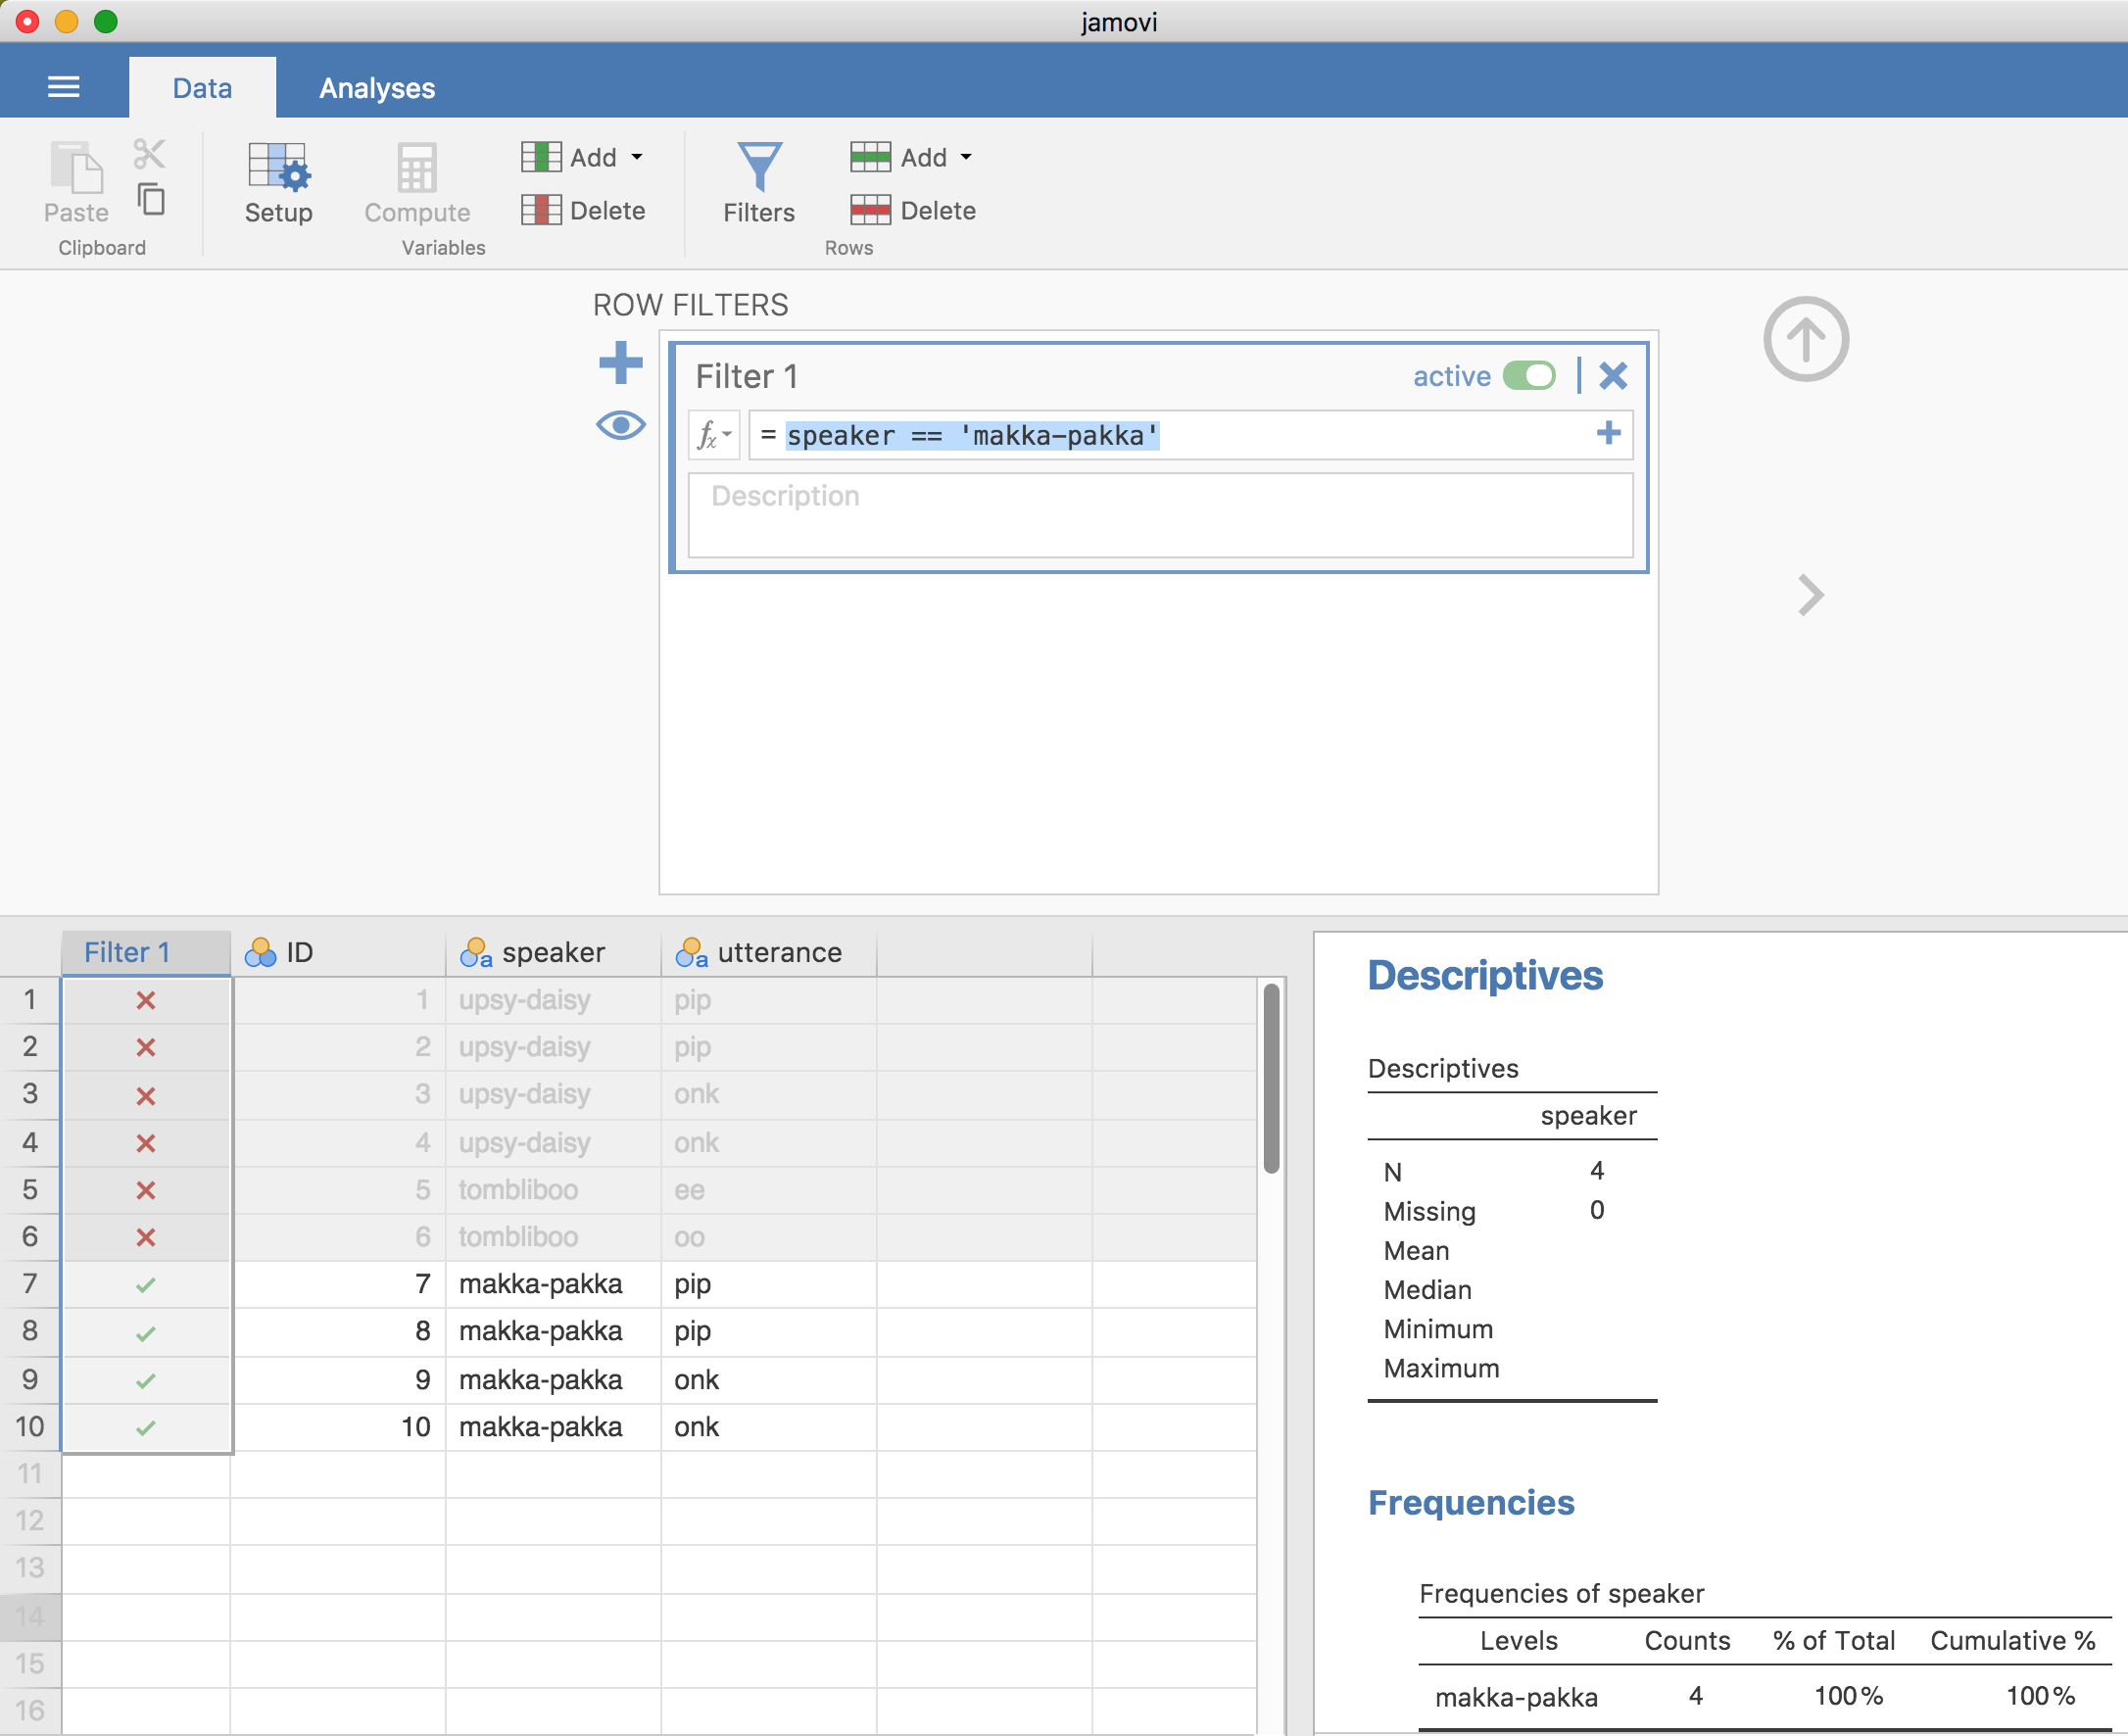
\epsfig{file = ../img/mechanics/subset1.png, clip=true,width =12cm} 
\caption{Creating a subset of the \rtext{nightgarden} data using the jamovi `Filters' option}
\label{fig:subset1}
\HR
\end{center}
\end{figure}

Following on from this simple example, you can also build up more complex filters using logical expressions in jamovi. For instance, suppose I wanted to keep only those cases when the utterance is either ``pip'' or ``oo''. In this case in the `Filter 1' text box, next to the `=' sign, you would type the following:

\begin{rblock1}
utterance == 'pip' or utterance == 'oo'
\end{rblock1}



%%%%%%%%%%%%%%%%%%%%%%%%%%%%%%%%%%%%%%%%%%%%
\begin{comment}
 - don't think this next section is required in jamovi



\section{Sorting, flipping and merging data~\label{sec:sort}}

In this section I discuss a few useful operations that I feel are loosely related to one another: sorting a vector, sorting a data frame, binding two or more vectors together into a data frame (or matrix), and flipping a data frame (or matrix) on its side. They're all fairly straightforward tasks, at least in comparison to some of the more obnoxious data handling problems that turn up in real life.




\section{Reshaping a data frame\label{sec:reshape}}




\SUBSECTION{Long form and wide form data}
The most common format in which you might obtain data is as a ``case by variable'' layout, commonly known as the \keyterm{wide form} of the data. 

\begin{rblock1}
> @usr{load("repeated.Rdata")}
> @usr{who()}
   -- Name --   -- Class --   -- Size --
   choice       data.frame    4 x 10    
   drugs        data.frame    10 x 8    
\end{rblock1}

To get a sense of what I'm talking about, consider an experiment in which we are interested in the different effects that alcohol and and caffeine have on people's working memory capacity (WMC) and reaction times (RT). We recruit 10 participants, and measure their WMC and RT under three different conditions: a ``no drug'' condition, in which they are not under the influence of either caffeine or alcohol, a ``caffeine'' condition, in which they are under the inflence of caffeine, and an ``alcohol'' condition, in which... well, you can probably guess. Ideally, I suppose, there would be a fourth condition in which both drugs are administered, but for the sake of simplicity let's ignore that. The \rtext{drugs} data frame gives you a sense of what kind of data you might observe in an experiment like this:
\begin{rblock1}
> @usr{drugs}
   id gender WMC_alcohol WMC_caffeine WMC_no.drug RT_alcohol RT_caffeine RT_no.drug
1   1 female         3.7          3.7         3.9        488         236        371
2   2 female         6.4          7.3         7.9        607         376        349
3   3 female         4.6          7.4         7.3        643         226        412
4   4   male         6.4          7.8         8.2        684         206        252
5   5 female         4.9          5.2         7.0        593         262        439
6   6   male         5.4          6.6         7.2        492         230        464
7   7   male         7.9          7.9         8.9        690         259        327
8   8   male         4.1          5.9         4.5        486         230        305
9   9 female         5.2          6.2         7.2        686         273        327
10 10 female         6.2          7.4         7.8        645         240        498
\end{rblock1}
This is a data set in ``wide form'', in which each participant corresponds to a single row. We have two variables that are characteristics of the subject (i.e., their \rtext{id} number and their \rtext{gender}) and six variables that refer to one of the two measured variables (WMC or RT) in one of the three testing conditions (alcohol, caffeine or no drug). Because all of the testing conditions (i.e., the three drug types) are applied to all participants, drug type is an example of a \keyterm{within-subject factor}. 


\SUBSECTION{Reshaping data using \rtext{wideToLong()}}

The ``wide form'' of this data set is useful for some situations: it is often very useful to have each row correspond to a single subject. However, it is not the only way in which you might want to organise this data. For instance, you might want to have a separate row for each ``testing occasion''. That is, ``participant 1 under the influence of alcohol'' would be one row, and ``participant 1 under the influence of caffeine'' would be another row. This way of organising the data is generally referred to as the \keyterm{long form} of the data. It's not too difficult to switch between wide and long form, and I'll explain how it works in a moment; for now, let's just have a look at what the long form of this data set looks like:
\begin{rblock1}
> @usr{drugs.2 <- wideToLong( data = drugs, within = "drug" )}
> @usr{drugs.2}
   id gender     drug WMC  RT
1   1 female  alcohol 3.7 488
2   2 female  alcohol 6.4 607
3   3 female  alcohol 4.6 643
4   4   male  alcohol 6.4 684
5   5 female  alcohol 4.9 593
6   6   male  alcohol 5.4 492
7   7   male  alcohol 7.9 690
8   8   male  alcohol 4.1 486
9   9 female  alcohol 5.2 686
10 10 female  alcohol 6.2 645
11  1 female caffeine 3.7 236
12  2 female caffeine 7.3 376

BLAH BLAH BLAH
\end{rblock1}
The \rtext{drugs.2} data frame that we just created has 30 rows: each of the 10 participants appears in three separate rows, one corresponding to each of the three testing conditions. And instead of having a variable like \rtextverb#WMC_caffeine# that indicates that we were measuring ``WMC'' in the ``caffeine'' condition, this information is now recorded in two separate variables, one called \rtext{drug} and another called \rtext{WMC}. Obviously, the long and wide forms of the data contain the same information, but they represent quite different ways of organising that information. Sometimes you find yourself needing to analyse data in wide form, and sometimes you find that you need long form. So it's really useful to know how to switch between the two.

In the example I gave above, I used a function called \rtext{wideToLong()} to do the transformation. The \rtext{wideToLong()} function is part of the \rtext{lsr} package. The key to understanding this function is that it relies on the {\it variable names} to do all the work. Notice that the variable names in the \rtext{drugs} data frame follow a very clear scheme. Whenever you have a variable with a name like \rtextverb#WMC_caffeine# you know that the variable being measured is ``WMC'', and that the specific condition in which it is being measured is the ``caffeine'' condition. Similarly, you know that \rtextverb#RT_no.drug# refers to the ``RT'' variable measured in the ``no drug'' condition. The measured variable comes first (e.g., \rtext{WMC}), followed by a separator character (in this case the separator is an underscore, \rtextverb#_#), and then the name of the condition in which it is being measured (e.g., \rtext{caffeine}). There are two different prefixes (i.e, the strings before the separator, \rtext{WMC}, \rtext{RT}) which means that there are two separate variables being measured. There are three different suffixes (i.e., the strings after the separtator, \rtext{caffeine}, \rtext{alcohol}, \rtext{no.drug}) meaning that there are three different levels of the within-subject factor. Finally, notice that the separator string (i.e., \rtextverb#_#) does not appear anywhere in two of the variables (\rtext{id}, \rtext{gender}), indicating that these are \keyterm{between-subject} variables, namely variables that do not vary within participant (e.g., a person's \rtext{gender} is the same regardless of whether they're under the influence of alcohol, caffeine etc).

Because of the fact that the variable naming scheme here is so informative, it's quite possible to reshape the data frame without any additional input from the user. For example, in this particular case, you could just type the following:
\begin{rblock1}
> @usr{wideToLong( drugs )}
   id gender   within WMC  RT
1   1 female  alcohol 3.7 488
2   2 female  alcohol 6.4 607
3   3 female  alcohol 4.6 643
4   4   male  alcohol 6.4 684

BLAH BLAH BLAH
\end{rblock1}
This is pretty good, actually. The only think it has gotten wrong here is that it doesn't know what name to assign to the within-subject factor, so instaed of calling it something sensible like \rtext{drug}, it has use the unimaginative name \rtext{within}. If you want to ensure that the \rtext{wideToLong()} function applies a sensible name, you have to specify the \rtext{within} argument, which is just a character string that specifies the name of the within-subject factor. So when I used this command earlier,
\begin{rblock1}
> @usr{drugs.2 <- wideToLong( data = drugs, within = "drug" )}
\end{rblock1}
all I was doing was telling \R\ to use \rtext{drug} as the name of the within subject factor. 

Now, as I was hinting earlier, the \rtext{wideToLong()} function is very inflexible. It {\it requires} that the variable names all follow this naming scheme that I outlined earlier. If you don't follow this naming scheme it won't work.\FOOTNOTE{This limitation is deliberate, by the way: if you're getting to the point where you want to do something more complicated, you should probably start learning how to use \rtextsmall{reshape()}, \rtextsmall{cast()} and \rtextsmall{melt()} or some of other the more advanced tools. The \rtextsmall{wideToLong()} and \rtextsmall{longToWide()} functions are included only to help you out when you're first starting to use R.} The only flexibility that I've included here is that you can change the separator character by specifying the \rtext{sep} argument. For instance, if you were using variable names of the form \rtext{WMC/caffeine}, for instance, you could specify that \rtext{sep="/"}, using a command like this
\begin{rblock1}
> @usr{drugs.2 <- wideToLong( data = drugs, within = "drug", sep = "/" )}
\end{rblock1}
and it would still work. 


\SUBSECTION{Reshaping data using \rtext{longToWide()}}

To convert data from long form to wide form, the \rtext{lsr} package also includes a function called \rtext{longToWide()}. Recall from earlier that the long form of the data (i.e., the \rtext{drugs.2} data frame) contains variables named \rtext{id}, \rtext{gender}, \rtext{drug}, \rtext{WMC} and \rtext{RT}. In order to convert from long form to wide form, all you need to do is indicate which of these variables are measured separately for each condition (i.e., \rtext{WMC} and \rtext{RT}), and which variable is the within-subject factor that specifies the condition (i.e., \rtext{drug}). You do this via a two-sided formula, in which the measured variables are on the left hand side, and the within-subject factor is on the ritght hand side. In this case, the formula would be \rtextverb#WMC + RT ~ drug#. So the command that we would use might look like this: 
\begin{rblock1}
> @usr{longToWide( data=drugs.2, formula= WMC+RT ~ drug )}
   id gender WMC_alcohol RT_alcohol WMC_caffeine RT_caffeine WMC_no.drug RT_no.drug
1   1 female         3.7        488          3.7         236         3.9        371
2   2 female         6.4        607          7.3         376         7.9        349
3   3 female         4.6        643          7.4         226         7.3        412
4   4   male         6.4        684          7.8         206         8.2        252
5   5 female         4.9        593          5.2         262         7.0        439
6   6   male         5.4        492          6.6         230         7.2        464
7   7   male         7.9        690          7.9         259         8.9        327
8   8   male         4.1        486          5.9         230         4.5        305
9   9 female         5.2        686          6.2         273         7.2        327
10 10 female         6.2        645          7.4         240         7.8        498
\end{rblock1}
or, if we chose to omit argument names, we could simplify it to this:
\begin{rblock1}
> @usr{longToWide( drugs.2, WMC+RT ~ drug )}
\end{rblock1}
Note that, just like the \rtext{wideToLong()} function, the \rtext{longToWide()} function allows you to override the default separator character. For instance, if the command I used had been 
\begin{rblock1}
> @usr{longToWide( drugs.2, WMC+RT ~ drug, sep="/" )}
\end{rblock1}
the output would contain variables with names like \rtext{RT/alcohol} instead of \rtextverb#RT_alcohol#.

\SUBSECTION{Reshaping with multiple within-subject factors}

As I mentioned above, the \rtext{wideToLong()} and \rtext{longToWide()} functions are quite limited in terms of what they can do. However, they do handle a broader range of situations than the one outlined above. Consider the following, fairly simple psychological experiment. I'm interested in the effects of practice on some simple decision making problem. It doesn't really matter what the problem is, other than to note that I'm interested in two distinct outcome variables. Firstly, I care about people's accuracy, measured by the proportion of decisions that people make correctly, denoted PC. Secondly, I care about people's speed, measured by the mean response time taken to make those decisions, denoted MRT. That's standard in psychological experiments: the speed-accuracy trade-off is pretty ubiquitous, so we generally need to care about both variables.

To look at the effects of practice over the long term, I test each participant on two days, \rtext{day1} and \rtext{day2}, where for the sake of argument I'll assume that \rtext{day1} and \rtext{day2} are about a week apart. To look at the effects of practice over the short term, the testing during each day is broken into two ``blocks'', \rtext{block1} and \rtext{block2}, which are about 20 minutes apart. This isn't the world's most complicated experiment, but it's still a fair bit more complicated than the last one. This time around we have two within-subject factors (i.e., \rtext{day} and \rtext{block}) and we have two measured variables for each condition (i.e., \rtext{PC} and \rtext{MRT}). The \rtext{choice} data frame shows what the wide form of this kind of data might look like: 
\begin{rblock1}
> @usr{choice}

  id gender MRT/block1/day1 MRT/block1/day2 MRT/block2/day1 MRT/block2/day2
1  1   male             415             400             455             450
2  2   male             500             490             532             518
3  3 female             478             468             499             474
4  4 female             550             502             602             588

  PC/block1/day1 PC/block1/day2 PC/block2/day1 PC/block2/day2
1             79             88             82             93
2             83             92             86             97
3             91             98             90            100
4             75             89             78             95
\end{rblock1}
Notice that this time around we have variable names of the form \rtext{MRT/block1/day2}. As before, the first part of the name refers to the measured variable (response time), but there are now two suffixes, one indicating that the testing took place in block 1, and the other indicating that it took place on day 2. And just to complicate matters, it uses \rtext{/} as the separator character rather than \rtextverb#_#. Even so, reshaping this data set is pretty easy. The command to do it is,
\begin{rblock1}
> @usr{choice.2 <- wideToLong( choice, within=c("block","day"), sep="/" )}
\end{rblock1}
which is pretty much the exact same command we used last time. The only difference here is that, because there are two within-subject factors, the \rtext{within} argument is a vector that contains two names. When we look at the long form data frame that this creates, we get this:
\begin{rblock1}
> @usr{choice.2}
   id gender MRT  PC  block  day
1   1   male 415  79 block1 day1
2   2   male 500  83 block1 day1
3   3 female 478  91 block1 day1
4   4 female 550  75 block1 day1
5   1   male 400  88 block1 day2
6   2   male 490  92 block1 day2

BLAH BLAH BLAH

15  3 female 474 100 block2 day2
16  4 female 588  95 block2 day2
\end{rblock1}
In this long form data frame we have two between-subject variables (\rtext{id} and \rtext{gender}), two variables that define our within-subject manipulations (\rtext{block} and \rtext{day}), and two more contain the measurements we took (\rtext{MRT} and \rtext{PC}). 

To convert this back to wide form is equally straightforward. We use the \rtext{longToWide()} function, but this time around we need to alter the formula in order to tell it that we have two within-subject factors. The command is now
\begin{rblock1}
> @usr{longToWide( choice.2, MRT+PC ~ block+day, sep="/" ) }
\end{rblock1}
and this produces a wide form data set containing the same variables as the original \rtext{choice} data frame. 


\SUBSECTION{What other options are there?}

The advantage to the approach described in the previous section is that it solves a quite specific problem (but a commonly encountered one) with a minimum of fuss. The disadvantage is that the tools are quite limited in scope. They allow you to switch your data back and forth between two different formats that are very common in everyday data analysis. However, there a number of other tools that you can use if need be. Just within the core packages distributed with \R\ there is the \rtext{reshape()} function, as well as  the \rtext{stack()} and \rtext{unstack()} functions, all of which can be useful under certain circumstances. And there are of course thousands of packages on CRAN that you can use to help you with different tasks. One popular package for this purpose is the \rtext{reshape} package, written by Hadley Wickham \cite<see>[for details]{Wickham2007}. There are two key functions in this package, called \rtext{melt()} and \rtext{cast()} that are pretty useful for solving a lot of reshaping problems. In a future version of this book I intend to discuss \rtext{melt()} and \rtext{cast()} in a fair amount of detail.


\end{comment}



\section{Loading and saving data\label{sec:load}}


There are several different types of files that are likely to be relevant to us when doing data analysis. There are two in particular that are especially important from the perspective of this book:
\begin{itemize}
\item {\it jamovi files} are those with a \filename{.omv} file extension. This is the standard kind of file that jamovi uses to store data, and variables and analyses. 
\item {\it Comma separated value (csv) files} are those with a \filename{.csv} file extension. These are just regular old text files, and they can be opened with almost any software. It's quite typical for people to store data in csv files, precisely because they're so simple.
\end{itemize} 

There are also several other kinds of data file that you might want to import into jamovi. For instance, you might want to open Microsoft Excel spreadsheets (\filename{.xls} files), or data files that have been saved in the native file formats for other statistics software, such as SPSS or SAS.  

Whichever file formats you are using, it's a good idea to create a folder or folders especially for your jamovi data sets and analyses, and to make sure you keep these backed up regularly. 

\SUBSECTION{Importing data from csv files}

One quite commonly used data format is the humble ``comma separated value'' file, also called a csv file, and usually bearing the file extension \filename{.csv}. csv files are just plain old-fashioned text files, and what they store is basically just a table of data. This is illustrated in Figure~\ref{fig:booksalescsv}, which shows a file called \filename{booksales.csv} that I've created. As you can see, each row represents the book sales data for one month. The first row doesn't contain actual data though: it has the names of the variables.

\begin{figure}
\begin{center}
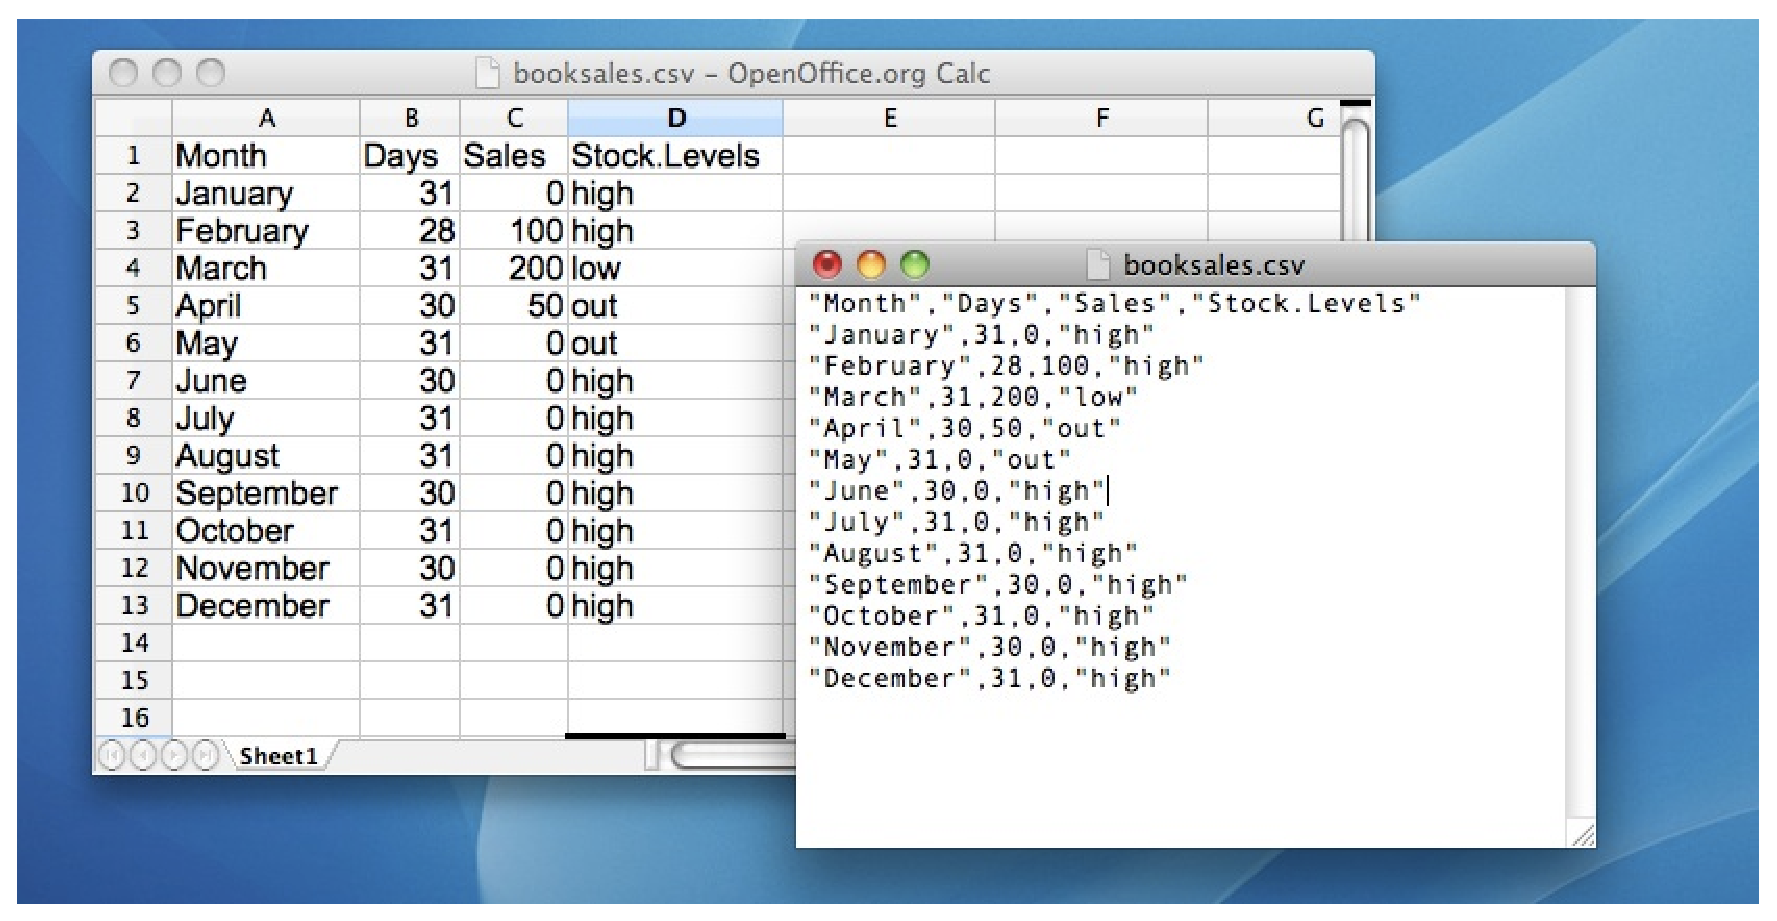
\epsfig{file = ../img/mechanics/booksalescsv.eps, clip=true,width = 14cm}
\caption{The \filename{booksales.csv} data file. On the left, I've opened the file using a spreadsheet program (OpenOffice), which shows that the file is basically a table. On the right, the same file is open in a standard text editor (the TextEdit program on a Mac), which shows how the file is formatted. The entries in the table are wrapped in quote marks and separated by commas.}
\HR
\label{fig:booksalescsv}
\end{center}
\end{figure} 

It's easy to open csv files in jamovi. From the top left menu (the button with three parallel lines) choose `Open' and browse to where you have stored the csv file on your computer. navigate to 




Click on that, and it will give you a couple of options: select the ``From Text File...'' option, and it will open up a very familiar dialog box asking you to select a file: if you're on a Mac, it'll look like the usual Finder window that you use to choose a file; on Windows it looks like an Explorer window. An example of what it looks like on a Mac is shown in Figure~\ref{fig:fileopen}. I'm assuming that you're familiar with your own computer, so you should have no problem finding the CSV file that you want to import! Find the one you want, then click on the ``Open'' button. When you do this, you'll see a window that looks like the one in Figure~\ref{fig:import}.

\begin{figure}[t]
\begin{center}
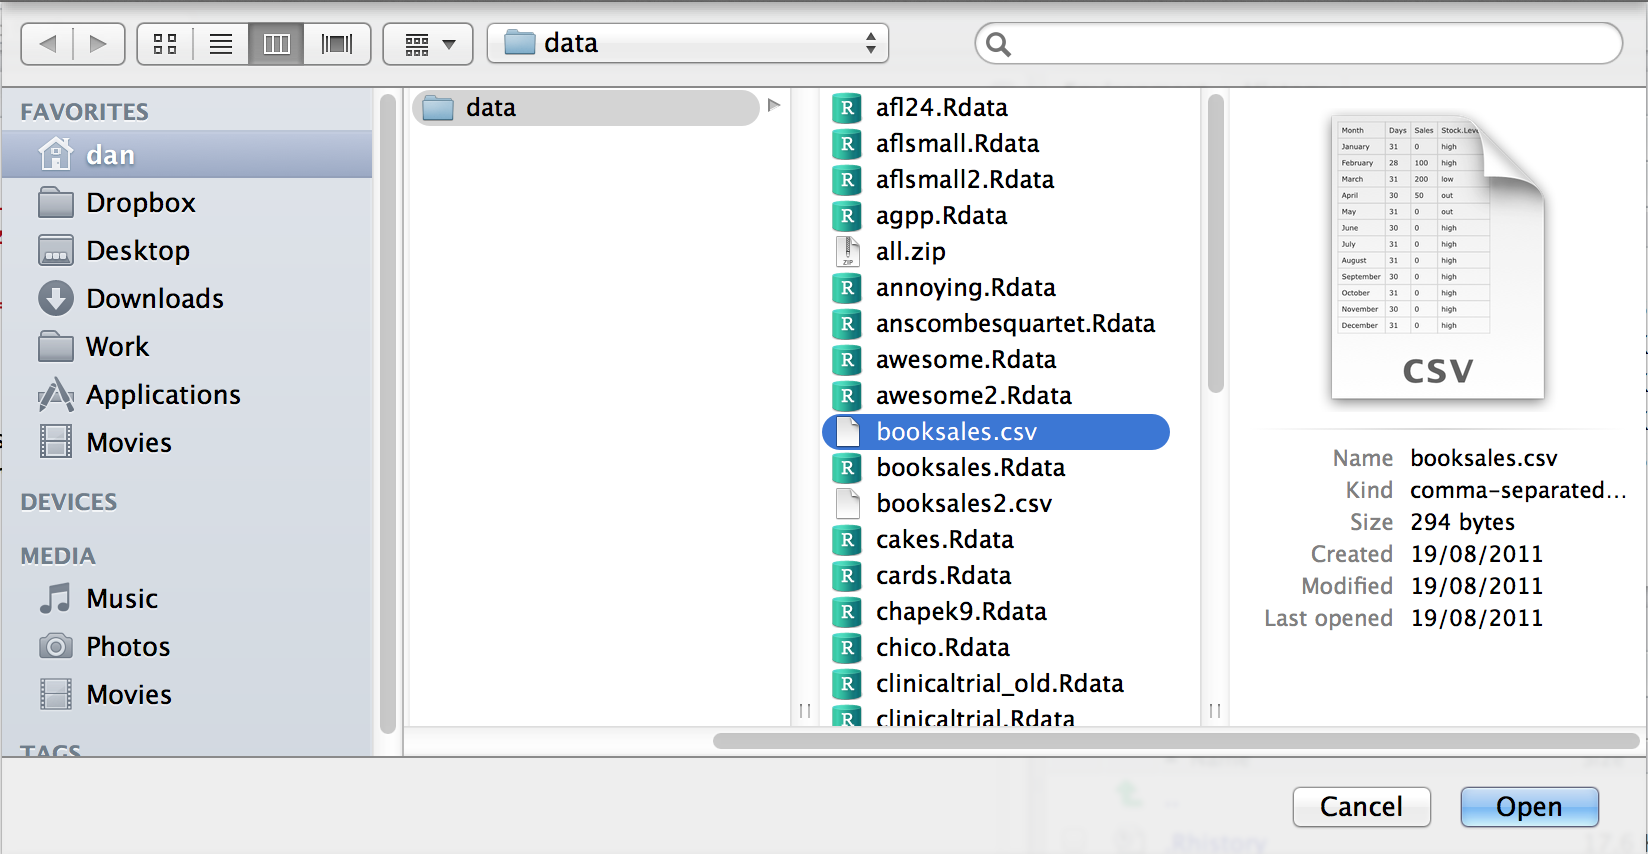
\epsfig{file = ../img/mechanics/openscreen.eps,clip=true, width = 14cm}
\caption{A dialog box on a Mac asking you to select the CSV file jamovi should try to import. Mac users will recognise this immediately: it's the usual way in which a Mac asks you to find a file. Windows users won't see this: they'll see the usual explorer window that Windows always gives you when it wants you to select a file.}
\HR
\label{fig:fileopen}
\end{center}
\end{figure} 

There are a few things that you can check to make sure that the data gets imported correctly: 

\begin{itemize}
\item Heading. Does the first row of the file contain the names for each variable - a `header' row? The \texttt{booksales.csv} file has a header, so that's a yes.
\item Separator. What character is used to separate different entries? In most csv files this will be a comma (it is ``comma separated'' after all).
\item Decimal. What character is used to specify the decimal point? In English speaking countries, this is almost always a period (i.e., \texttt{.}). That's not universally true: many European countries use a comma. 
\item Quote. What character is used to denote a block of text? That's usually going to be a double quote mark. It is for the \texttt{booksales.csv} file.
\end{itemize}


\section{Importing unusual data files~\label{sec:importing}}

Throughout this book I've assumed that your data are stored as a jamovi \filename{.omv} file or as a ``properly'' formatted csv file. However, in real life that's not a terribly plausible assumption to make, so I'd better talk about some of the other possibilities that you might run into. 


\SUBSECTION{Loading data from text files} 

The first thing I should point out is that if your data are saved as a text file but aren't {\it quite} in the proper csv format, then there's still a pretty good chance that jamovi will be able to open it. You just need to try it and see if it works. Sometimes though you will need to change some of the formatting. The ones that I've often found myself needing to change are:
\begin{itemize}
\item \rtext{header}. A lot of the time when you're storing data as a csv file, the first row actually contains the column names and not data. If that's not true, then it's a good idea to open up the csv file in a spreadsheet programme such as Open Office and add the header row manually. 
\item \rtext{sep}. As the name ``comma separated value'' indicates, the values in a row of a csv file are usually separated by commas. This isn't universal, however. In Europe the decimal point is typically written as \rtext{,} instead of \rtext{.} and as a consequence it would be somewhat awkward to use \rtext{,} as the separator. Therefore it is not unusual to use \rtext{;} instead of \rtext{,} as the separator. At other times, I've seen a TAB character used. 
\item \rtext{quote}. It's conventional in csv files to include a quoting character for textual data. As you can see by looking at the \filename{booksales.csv} file, this is usually a double quote character, \rtext{"}. But sometimes there is no quoting character at all, or you might see a single quote mark \rtext{'} used instead. 
\item \rtext{skip}. It's actually very common to receive CSV files in which the first few rows have nothing to do with the actual data. Instead, they provide a human readable summary of where the data came from, or maybe they include some technical info that doesn't relate to the data. 
\item \rtext{missing values}. Often you'll get given data with missing values. For one reason or another, some entries in the table are missing. The data file needs to include a ``special'' value to indicate that the entry is missing. By default jamovi assumes that this value is \rtext{99}\FOOTNOTE{You can change the default value for missing values in jamovi from the top right menu (three vertical dots), but this only works at the time of importing data files into jamovi}, for both numeric and text data, so you should make sure that, where necessary, all missing values in the csv file are replaced with \rtext{99} before opening / importing the file into jamovi. Once you have opened / imported the file into jamovi all the \rtext{99} missing values are converted to blank cells in the jamovi spreadsheet view.
\end{itemize}


\SUBSECTION{Loading data from SPSS (and other statistics packages)}

The commands listed above are the main ones we'll need for data files in this book. But in real life we have many more possibilities. For example, you might want to read data files in from other statistics programs. Since SPSS is probably the most widely used statistics package in psychology, it's worth mentioning that jamovi can also import SPSS data files (file extension \filename{.sav}). Just follow the instructions above for how to open a csv file, but this time navigate to the .sav file you want to import. Again, jamovi will regard all values as missing according to its `Default missings' value.

And that's pretty much it, at least as far as SPSS goes.  As far as other statistical software goes, jamovi can also directly open / import SAS and STATA files. 


\SUBSECTION{Loading Excel files} 

A different problem is posed by Excel files. Despite years of yelling at people for sending data to me encoded in a proprietary data format, I get sent a lot of Excel files. The way to handle Excel files is to open them up first in Excel or another spreadsheet programme that can handle Excel files, and then export the data as a csv file, before opening / importing the csv file into jamovi. 


\section{Changing data from one level to another\label{sec:coercion}}

Sometimes you want to change the variable level. This can happen for all sorts of reasons. Sometimes when you import data from files, it can come to you in the wrong format: numbers sometimes get imported as nominal, text values. Dates may get imported as text. Nominal values can sometimes be read as ordinal or even continuous. There's a good chance that sometimes you'll want to convert a variable from one measurement level into another one. Or, to use the correct term, you want to \keyterm{coerce} the variable from one class into another. 

In \ref{sec:spreadsheet} we saw how to specify different variable levels, and if you want to change a variable's measurement level then you can do this in the jamovi data view for that variable. Just click the check box for the measurement level you want - continuous, ordinal, or nominal. 


\section{Summary}

Obviously, there's no real coherence to this chapter. It's just a grab bag of topics and tricks that can be handy to know about, so the best wrap up I can give here is just to repeat this list:

\begin{itemize} \itemsep 0pt
\item Section~\ref{sec:freqtables}. Tabulating data.
\item Section~\ref{sec:transform}. Transforming or recoding a variable.
\item Section~\ref{sec:mathfunc}. Some useful mathematical functions.
\item Section~\ref{sec:subset}. Extracting a subset of a vector.
\item Section~\ref{sec:textprocessing}. Manipulating text.
\item Section~\ref{sec:importing}. Opening data from different file types.
\item Section~\ref{sec:coercion}. Coercing data from one type to another.
\item Section~\ref{sec:datastructures}. Other important data types.
\item Section~\ref{sec:miscdatahandling}. Miscellaneous topics.
\end{itemize}



